\section{Algoritmos y aplicaciones}

Dado el problema planteado, su solucion implica el uso de algoritmos de vision por computadora.

\subsection{Redes Neuronales Convolucionales (CNNs)}

Las redes neuronales convolucionales (CNN) son una alternativa especialmente
adecuada para este problema debido a su capacidad para procesar información
espacial. Mediante filtros convolucionales pueden aprender automáticamente
características de las imágenes, como bordes, texturas y formas. En las capas
internas pueden emplearse funciones de activación como ReLU, mientras que
Softmax puede utilizarse en la salida para representar las probabilidades de
las distintas clases.

\begin{figure}[htbp]
    \centering
    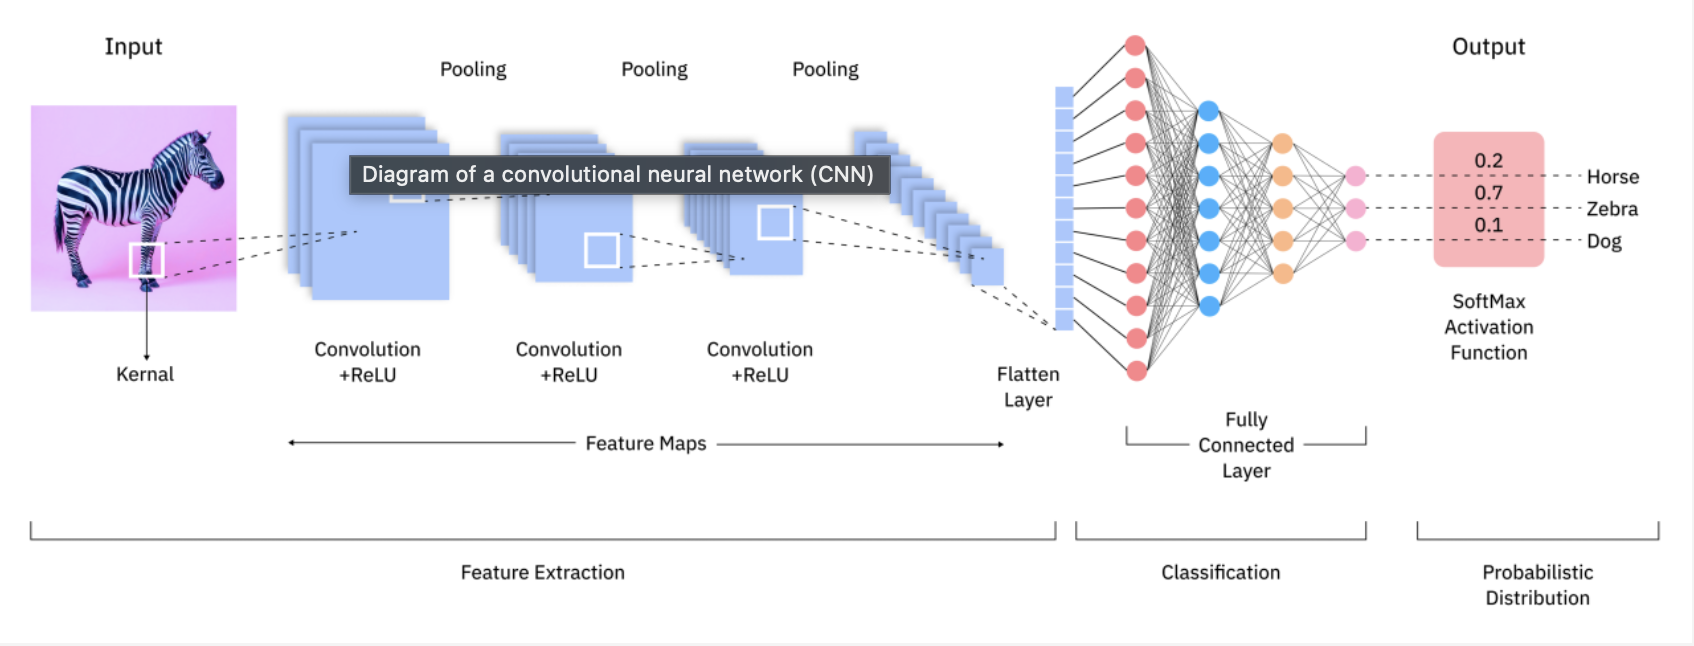
\includegraphics[width=\columnwidth]{cnn_diagram.png}
    \caption{La convolución descompone la imagen en caracteristicas para aprender a clasificar \autocite{ibmWhatImage}.}
    \label{fig:cnn_diagram}
    
\end{figure}


Este método parece ser el principal y el mejor para producir resultados optimos, aunque, dado a la gran cantidad de datos que se tienen que tratar y la variedad de operaciones que se llevan a cabo, hay que considerar que es un metodo lento y computacionalmente pesado. Esto habilita la posibilidad de usar otros algoritmos que se ajusten a la necesidad del problema.

\subsection{Otros algoritmos sin aprendizaje profundo}


\begin{description}
    \item[k vecinos más cercanos (KNN)] Cada imagen lo representa como un vector de características. Usa normalmente la distancia euclidiana para medir las similaridades entre los puntos, y compara con sus k vecinos más cercanos para clasificar la imagen. Es un algoritmo de aprendizaje supervisado.
    \item[Bosque aleatorio] Se compone de un conjunto de árboles de decisión, se calcula la media de los resultados de los árboles.
    \item[Máquinas de Vectores de Soporte (SVMs)] Este algoritmo encuentra la línea óptima para separar dos clases. Una variación llamada SVM multiclase existe para problemas multiclase, como este contexto.
\end{description}


\subsection{Otros modelos de aprendizaje profundo}

\begin{description}
    \item[ResNet] Conocida también como \textit{Residual network}. Útil para entrenar redes neuronales muy profundas. La cota superior para implementar este método es la capacidad de nuestro \textit{hardware} o acceso a equipo computacional que sea capaz de entrenar este tipo de redes más complejas.
    \item[Otros modelos ya implementados] Como \textbf{AlexNet} o \textbf{GoogleNet/inception} que tienen una gran capacidad para reconocer y clasificar imágenes.\autocite{ibmWhatImage}
\end{description}


\subsection{Aplicaciones posibles}

Un modelo capaz de clasificar tipos de flores a partir de imágenes puede tener distintas aplicaciones reales. Una de ellas es la \textbf{identificación automática de plantas}, donde un usuario podría tomar una fotografía y recibir como resultado la especie o clase más probable.


Un ejemplo de este tipo de aplicaciones yace en el apoyo a plataformas de ciencia ciudadana y el monitoreo de biodiversidad. Por ejemplo, iNaturalist ha acumulado más de 300 millones de observaciones hechas por personas comunes \autocite{inaturalist} y utiliza un modelo de visión por computadora, entrenado con esas mismas observaciones, para sugerir la especia a partir de una fotografía. Sin este apoyo automático, cada observación dependería de que una persona la revisara detenidamente, lo que haría el proceso lento y difícil de escalar. Automatizar parte de la tarea ayuda a mejorar la eficiencia y aporta de gran manera a la obtención de datos sobre biodiversidad. Este proyecto es una versión a menor escala de este tipo de sistemas. 

Otra aplicación sería como \textbf{herramienta educativa}, por ejemplo, en aplicaciones para estudiantes o visitantes de jardines botánicos que permitan reconocer flores y consultar información sobre ellas.

Sin embargo, el modelo desarrollado solo podría reconocer las 104 clases presentes en el conjunto de datos, por lo que una aplicación real más amplia requeriría entrenarlo con una mayor variedad de especies.
